
\documentclass{elsarticle}
\journal{Artificial Intelligence Journal}
\usepackage{bm,url,amsmath,amssymb}
%\usepackage{boldsymbol}
\usepackage{color,colortbl} % for \todo command
\usepackage{verbatim} % for \begin{comment}'ing out sections.
\usepackage{algorithm,algorithmicx}
\usepackage{algpseudocode}
\usepackage{mathtools}

\DeclarePairedDelimiter\ceil{\lceil}{\rceil}
\DeclarePairedDelimiter\floor{\lfloor}{\rfloor}

% For revision history
\newcommand{\vcpath}{vc.tex}

\IfFileExists{\vcpath}{\input{\vcpath}}{
	\newcommand{\giturl}{UNKNOWN}
	\newcommand{\gitslug}{UNKNOWN}
	\newcommand{\githash}{UNKNOWN}
	\newcommand{\gitdate}{UNKNOWN}
	\newcommand{\gitauthor}{UNKNOWN}
}


\newcommand{\todo}[1]{\textcolor{red}{#1}}
\usepackage[T1]{fontenc}
\newcommand{\nbb}[2]{
    % \fbox{\bfseries\sffamily\scriptsize#1}
    \fcolorbox{black}{cyan}{\bfseries\sffamily\scriptsize#1}
    {\sf$\blacktriangleright$\textcolor{blue}{\textit{#2}}$\blacktriangleleft$}
    % \marginpar{\fbox{\bfseries\sffamily#1}}
}

\newcommand{\nbt}[2]{
    % \fbox{\bfseries\sffamily\scriptsize#1}
    \fcolorbox{black}{red}{\bfseries\sffamily\scriptsize#1}
    {\sf$\blacktriangleright$\textcolor{blue}{\textit{#2}}$\blacktriangleleft$}
    % \marginpar{\fbox{\bfseries\sffamily#1}}
}
\newcommand{\nbd}[2]{
    % \fbox{\bfseries\sffamily\scriptsize#1}
    \fcolorbox{black}{green}{\bfseries\sffamily\scriptsize#1}
    {\sf$\blacktriangleright$\textcolor{blue}{\textit{#2}}$\blacktriangleleft$}
    % \marginpar{\fbox{\bfseries\sffamily#1}}
}
\newcommand{\alda}[1]{\nbb{Aldeida}{#1}}
\newcommand{\andy}[1]{\nbb{Andy}{#1}}


% Define commands
\newcommand{\article}{\emph{Article}}
\newcommand{\acronym}[1]{{\small{#1}}}
\newcommand{\project}[1]{\textsl{#1}}

% Surveys
\newcommand{\apogee}{\acronym{APOGEE}}
\newcommand{\ges}{\acronym{GES}}
\newcommand{\hermes}{\acronym{HERMES}}
\newcommand{\galah}{\acronym{GALAH}}
\newcommand{\fourmost}{\acronym{4MOST}}
\newcommand{\weave}{\acronym{WEAVE}}
\newcommand{\gaia}{\project{Gaia}}
\newcommand{\Cspace}{$\mathcal{C}$-space }
\newcommand{\Cspaceno}{$\mathcal{C}$-space}

% Common terms
\newcommand{\vect}[1]{\boldsymbol{\mathbf{#1}}}
\renewcommand{\vec}[1]{\vect{#1}}

\def\teff{T_{\rm eff}}
\def\logg{\log{g}}

% Have some maaaath.
\def\transpose{^\intercal}
\def\infinity{\rotatebox{90}{8}}
\def\cov{C}
\def\veccov{\vect{\cov}}
\def\vecmean{\vect{\mu}}
\def\vectheta{\vect{\theta}}
\def\weight{w}
\def\weights{\vect{\weight}}
\def\datum{y}
\def\data{\vect{\datum}}
\def\likelihood{\mathcal{L}}
\newcommand{\fisher}[1]{\mathcal{F}\left(#1\right)}
\newcommand{\detfisher}[1]{\left|\fisher{#1}\right|}
\newcommand{\prior}[1]{p\left(#1\right)}

\newcommand{\bashcommand}[1]{\noindent\texttt{#1}\\}


% Affiliation(s)
\newcommand{\moca}{
    \affil{School of Physics and Astronomy, Monash University, 
        Melbourne, Clayton VIC 3800, Australia}}
\newcommand{\claytonfit}{
    \affil{Faculty of Information Technology, Monash University,
        Melbourne, Clayton VIC 3800, Australia}}
\newcommand{\caulfieldfit}{
    \affil{Faculty of Information Technology, Monash University,
        Melbourne, Caulfield East VIC 3145, Australia}}



\begin{document}
    \begin{frontmatter}
%       \title{Searching for the Origins of the Galaxy with the Minimum Message Length}
%       \title{Searching for the Origins of the Galaxy with Minimum Message Length mixture modelling}
%        \title{Reconstructing the Origins of the Galaxy with Minimum Message Length mixture modelling and new search techniques}
        \title{Search techniques for gaussian mixture modelling with Minimum Message Length, with applications to the origin of our Galaxy}
        
%% Group authors per affiliation:
\author[fit]{Aldeida Aleti\corref{mycorrespondingauthor}}
\cortext[mycorrespondingauthor]{Corresponding author}
\ead{aldeida.aleti@monash.edu}
\author[moca,fit]{Andrew R. Casey}
\author[moca]{John C. Lattanzio}
\author[fit]{David L. Dowe}
\address[moca]{School of Physics and Astronomy, Monash University, Melbourne, Clayton VIC 3800, Australia}
\address[fit]{Faculty of Information Technology, Monash University, Melbourne, Clayton VIC 3800, Australia}

        
        \begin{abstract}

        
        \end{abstract}
        
        
        \begin{keyword}
            Search\sep Minimum Message Length\sep MML\sep gaussian mixture models\sep Galactic Archaeology
        \end{keyword}
    \end{frontmatter}
\section{Introduction} 
\label{sec:introduction}

The contributions of this paper are:
\begin{itemize}
\item Solving the galactic archaeology (GA) problem using mixture modelling
% bear in mind or don't forget that GA will mean `genetic algorithms' to many readers
\item Minimum Message Length (MML) formulation
\item $\mathcal{O}\left(K\right)$ search methods for gaussian mixture  modelling
\end{itemize}
\section{Galactic Archaeology}
Galactic Archaeology~\cite{freeman2002new} aims at reconstructing the history 
of our galaxy by identifying ancient star formation events. Most stars are 
born in clusters (of order $10^0$ to $10^6$ stars at a time), and all approximately
share the same chemical composition of the gas cloud that they form from.
Stars in clusters often do not remain gravitationally bound, and disperse 
throughout the disk of our galaxy within about $10^9\,{\rm yr}$. %citation needed.
As a consequence, where a star is now does not reflect its formation site, 
which complicates our understanding of galaxy formation and evolution. However, the
observable chemical composition of a star remains largely the same throughout
that star's lifetime, providing an immutable marker (a chemical tag, or
`fingerprint') that carries with it information about where and when every star
formed.


Observations reveal that stars in surviving clusters show very little scatter
in their chemical composition~\cite{pancino2010chemical}, and that star
clusters can be identified solely on the basis of stellar chemical
abundances~\cite{Hogg:2016}. Astronomers have precisely measured the
chemical composition for hundreds of thousands of stars in the disk of our galaxy,
where the natal formation site for most stars is not known~\cite{Buder:2018}.
Indeed, from those data it is not known how many star formation sites we might
expect to be able to detect, and we do not know the number of stars that we
might to observe from each cluster (the so-called stellar mass function).
Theoretical simulations can provide a guide to these quantities, but the
predictions are still uncertain.
% large variance.


These facts conspire to produce a challenging parameter estimation and model
selection problem that is analagous to mixture modelling, where the true number 
of mixtures is unknown. Little work has been done to address this problem so 
far, apart from the work of \cite{mitschang2014quantitative}, who used the 
\emph{Manhattan distance} metric to quantify the chemical difference between 
any two stars, and estimate the level of homogeneity expected within a cluster. 
This metric calculates the mean weighted absolute difference of abundance 
levels, $\sigma_C$, between two stars $S^a$ and $S^b$ as follows:
% Given that $\sigma$ is so widely used to mean standard deviation, this notation 
% (to follow) seems a bit unfortunate
$\sigma_C = \sum_{c \in C}w_c|S^a_c-S^b_c|/||C||$, where $C$ is the set of 
chemical species, $S^a_c$ is the chemical abundance of element $c$ in star $
S^a$, $w_c$ is the weight given to species $c$, and $||C||$ is the total 
number of chemical species\footnote{Here we describe the work of Mitschang et
al. (2014)~\cite{mitschang2014quantitative} using their notation, but we 
caution that we use similar notation in this work with very different 
terminology and meaning.}. The Manhattan distance values are high for stars 
from different clusters, and low for stars from the same cluster. Note that 
this metric is not particularly robust or versatile; for example it is not 
invariant even to a simple rotation of the co-ordinate axes.
% - and nor does it take into account that a difference between two stars of (say) 0.01\% in a rare element might be
% vastly more significant than the same difference in a vastly more abundant element
% Retraction.  It does endeavour to take that into account, via the weights, $w_c$, but not by setting them all to 1.
An important issue is how to set the weights for each chemical species $w_c$, 
and how they affect the results (Mitschang et al.~\cite{mitschang2014quantitative} 
used $w_c=1$). Another issue is setting the boundary between clusters. It is 
not clear what a high and low Manhattan distance is; these values are subjective. 
In this paper, we express the problem in terms of mixture modelling and infer 
the number of clusters, their mixing proportions (or relative abundances) and 
each cluster's statistical distribution using Minimum Message Length (MML) and 
novel search techniques that are readily applicable to the large data sets
being accumulated by astronomers worldwide.


% Not clear how many star formation sites, etc...

%and using that as a reflection from the gas cloud that those stars
%formed. Through successive generations of star formation, each fusing light
%elements into heavy ones and releasing them into the interstellar medium,
%the chemical composition of a star-forming gas cloud reflects the lives and
%deaths of previous generations of stars. 

% accreted by our own Galaxy during its youth. This is possible because stars form in clusters of 10s to 1000s at a time, all sharing the same composition, being that of the gas cloud from which they formed. This composition is due to the action of previous generations of stars in fusing light elements into heavy ones, and leads an improved understanding of nuclear processes in stars.
%and which stars they operate in.

%The idea of Galactic Archaeology relies on identifying stars born together based on their composition. Internal mechanisms change the abundance of the lighter elements, but the heavier ones remain mostly unchanged. These provide a ``chemical tag'' or a ``stellar DNA'' that can be used to identify the stars. 

%Observations have shown that each star cluster has a uniform and distinct chemical fingerprint~\cite{pancino2010chemical}. Our aim is to identify stars with the same composition, as these
% were
%are widely believed to have been
%almost certainly
%formed at the same time in the same cluster. We expect this cluster has now dispersed, but the tell-tale chemical tags will be present and will allow us to identify the groups of stars that are the relics of ancient star forming activity.

%Little work  has been done to address this problem so far, apart from the work of \cite{mitschang2014quantitative}, who used the \emph{Manhattan distance} metric to  quantify the chemical difference between any two stars, and as a result estimate the level of homogeneity expected within a cluster. This metric calculates the mean weighted absolute difference of abundance levels, $\sigma_C$, between two stars $S^a$ and $S^b$ as follows:
%% Given that $\sigma$ is so widely used to mean standard deviation, this notation (to follow) seems a bit unfortunate
%$\sigma_C = \sum_{c \in C}w_c|S^a_c-S^b_c|/||C||$, where $C$ is the set of chemical species, $S^a_c$ is the chemical abundance of element $c$ in star $S^a$, $w_c$ is the weight given to species $c$, 
%which is considered 1 for all elements in the current work, 
%and $||C||$ is the total number of chemical species. The Manhattan distance values are high for stars from different clusters, and low for stars from the same cluster. Note that this metric is not particularly robust or versatile; for example it is not even invariant to a simple rotation of the co-ordinate axes
% - and nor does it take into account that a difference between two stars of (say) 0.01\% in a rare element might be
% vastly more significant than the same difference in a vastly more abundant element
% Retraction.  It does endeavour to take that into account, via the weights, $w_c$, but not by setting them all to 1.
%An important issue is how to set the weights for each chemical species $w_c$, and how they affect 
%the results (Mitschang et al.~\cite{mitschang2014quantitative} used $w_c=1$). Another issue is setting the boundary between clusters. It is not clear what a high and low Manhattan distance is; at the moment 
%these values are largely subjective. In this paper, we express the problem in terms of mixture modelling and infer the number of clusters, their mixing proportions (or relative abundances) and each cluster's statistical distribution using Minimum Message Length (MML) and two novel search techniques.  

\section{Related Work in Mixture Modelling}

\noindent{}Mixture modelling is composed of three main parts:
\begin{enumerate}
    \item an estimator of component parameters of a mixture;
    \item an objective functions that scores a mixture; and 
    \item a search strategy which identifies the best number of components and
          their relative weights.
\end{enumerate}

Different criteria for estimating component parameters have been used in the 
literature, with traditional methods using maximum likelihood estimation (MLE)
% Perhaps because ML could refer to many things (e.g., machine learning), maximum likelihood is often (I think usually) called MLE
~\cite{akaike1971determination} or maximum a posteriori probability (MAP)~\cite{shimony1994finding}.
These methods do not consider the complexity of the model, but only focus on
the goodness-of-fit, and require modification to minimise the risk of
over-fitting. In this work, we focus on the Bayesian information-theoretic 
Minimum Message Length (MML) principle~\cite{WallaceBoulton1968, WallaceFreeman1987, WallaceDowe1999a, Wallace:2005}.
Unlike MLE or MAP estimators, the MML principle is invariant under non-linar
data transformations, and can seemlessly incorporate different probability
distributions.



%have not been designed to consider the complexity of the model, but only focus on the goodness-of-fit. They have to be modified with ad-hoc principles in order to ensure that the data is not over-fitted. This is a very important property for astrophysical applications. 
%
% In this work, we focus on the Bayesian Minimum Message Length Principle~\cite{Wallace:2005}, which unlike MAP estimators, are invariant under non-linear data transformations.
%, and different from MLE, can be used with different probability distributions.  
%
The classically-described princple of MML is that the best explanation of the
data is the one that leads to the shortest so-called two-part message~\cite{Wallace:2005}, 
where a \textit{message} takes into account both the complexity of the model 
and its explanatory power. The complexity of the model is described through
the first part of the message, and the second part of the message describes
its explanatory power. The \emph{length} of each message part is quantified
(or measured) using information theory, allowing for a fair evaluation between
different models of varying complexity or explanatory power. MML has been 
shown to perform well on a variety of empirical analyses (see, e.g., 
\cite{viswanathan1999finding,fitzgibbon2004minimum}, with references to 
further examples in \cite{Wallace:2005,dowe2007bayes,Dowe2008a,Dowe2011a}).


% ARC: Not sure if this paragraph should be here...
Arguments about the statistical consistency (i.e.,~as the number of data 
points increases the distributions of the estimates become increasingly 
concentrated near the true value) of MML are given in \cite{DoweWallace1997a,Dowe2011a}.
The MML principle requires that we explicitly specify our prior beliefs on the
model parameters, providing a Bayesian optimisation approach which can be
applied across entire classes of models.

%Unlike the rival Bayesian approach MAP, for continuous parameters MML is a statistically invariant (meaning that $1$-to-$1$ transformations of co-ordinates, such as polar $(r, \theta)$ to Cartesian $(x, y)$, leave the answer unchanged) Bayesian approach~\cite{WallaceFreeman1987,WallaceDowe1999a,Wallace:2005,dowe2007bayes}. It allows the modelling of prior beliefs in the calculation of the best model parameters. If one has a particular reason to expect one value rather than another, a prior probability can be chosen to represent that belief. Of course, we can also model the data as objectively as Bayesianism permits. 

Two other well-known methods based on information theory are the Akaike 
Information Criterion (AIC)~\cite{akaike1974} and Bayesian Information Criterion
(BIC)~\cite{schwarz1978estimating}, both of which endeavour to temper maximum 
likelihood's tendency to over-fit and under-estimate the noise. Unlike maximum
likelihood, MML accounts for model complexity, and for this reason maximum
likelihood can be thought of as MML without including the first part of the
message that describes the model complexity. AIC~\cite{akaike1974} chooses a 
model with the motivation of minimizing the Kullback-Leibler divergence 
between the model and the truth:
% KL divergence is generally asymmetric
\begin{equation}
    AIC = -2 \log_{e}f(\vec{\data} | \vec{\theta}) + 2 k
\end{equation}
\noindent{}where the likelihood $f(\vec{\data} | \vec{\theta})$ is the probability 
of the data $\vec{\data}$ given a model parameterised by $\vec{\theta}$, and $k$ 
is the number of free parameters in the model. BIC~\cite{schwarz1978estimating} 
uses a constant penalty equal to $\frac{1}{2}\log{N}$ for each free parameter in the 
model, where $N$ is the number of data points. Minimum Description Length (MDL)
~\cite{rissanen1978modeling} is a similar approach to BIC~\cite{schwarz1978estimating},
and has close (albeit also distinct) ties to MML \cite{WallaceBoulton1968}.
AIC and BIC/MDL associate parameter costs (or model complexity) with the number 
of free parameters, not the values of those parameters or the variance that
can be explained by those parameters. As a result, when using AIC or BIC/MDL
formalisms, all models of a particular probability distribution share the same
cost, regardless of their respective means, covariance matrices, or the
Fisher information, which could bias inferences.


% Comparisons of MML to other methods
% clearly indicate MML's theoretical and empirical superiority.
% Let's not overly annoy the reviewers and readers.
%Examples of MML's promise against rival methods include comparisons with AIC~\cite{dowe2007bayes}, BIC \cite{agusta2002mml}, MDL~\cite{viswanathan1999finding} and MLE~\cite{dowe2007bayes} - and also in statistical econometric time series autoregression \cite{fitzgibbon2004minimum}, machine learning problems \cite{viswanathan1999finding},
%angular data \cite{WallaceDowe1993,DoweOliverWallace1996}
%and using this modelling \cite{WallaceDowe1993} to infer the order in which various parts of a protein fold~\cite{edgoose1998mml}. 

%A further example is the problem of deciding whether or not some 1-dimensional data generated uniformly in the interval $[ 0, 1 ]$ has a gap in it. Curiously, even when there is clearly no gap, AIC infers that there is a gap, whereas MML gives the right answer \cite{dowe2007bayes}. 

%Very importantly, the MML message structure enables us to robustly deal with missing data \cite{WallaceDowe1994b,WallaceDowe1997,WallaceDowe2000}. Other methods often replace missing values with the mean - in turn, reducing the true standard deviation - or various other imputed methods. In MML, on the other hand, missing data can easily be left out from the calculations from modelling done so far, simply encoding the missing data as missing \cite{WallaceDowe1994b,WallaceDowe1997a,WallaceDowe2000}, which is very useful when modelling astrophysical data, where missing observations are quite common.

The parameters of a mixture model can be estimated using Expectation-Maximisation 
(EM)~\cite{dempster1977maximum}. The EM algorithm has been used with MML to 
infer Gaussian mixtures under different simplifying assumptions, such as 
assuming that the covariance matrices are diagonal~\cite{WallaceDowe1994b, WallaceDowe1997a, WallaceDowe2000} 
(where it is sometimes called an `adjust cycle') and \cite{oliver1996unsupervised},
or approximating the probabilities of mixture parameters~\cite{figueiredo2002unsupervised,roberts1998bayesian}. 
The search algorithm employed in the majority of these approaches is based on 
running EM iteratively for different numbers of components~\cite{WallaceDowe1994b, 
WallaceDowe1997a, WallaceDowe2000, oliver1996unsupervised,roberts1998bayesian,
biernacki2000assessing}. The search method proposed by Figueiredo and Jain
~\cite{figueiredo2002unsupervised}, on the other hand, starts with a large 
number of components, and iteratively deletes components. A mirror extension 
of this method was proposed by Kasarapu and Allison~\cite{Kasarapu|Allison:2015}, 
which starts with one components, and selectively splits, deletes, or merges 
components in an attempt to minimise the message length. While this method 
removes the overhead introduced by the search algorithm of Figueiredo and Jain
~\cite{figueiredo2002unsupervised}, the search remains greedy, and can be 
prone to premature convergence in suboptimal solutions. The search methods 
introduced in this paper, incorporate a perturbation step which encourages 
explorations of new local optima.

%{\color{blue}References that we/you seem to be missing include
%\cite{WallaceBoulton1968, WallaceFreeman1987, WallaceDowe1999a}
%% these three above are probably the three most-cited MML papers
%and
%WallaceDowe1993,WallaceDowe1994b,DoweOliverWallace1996,
% these three works above are the earliest MML works on angular data and mixture modelling with angular data
%DoweWallace1997
%% the above is a work about MML statistical consistency
%WallaceDowe1997,WallaceDowe2000
% these two papers above are MML mixture modelling papers
%Dowe2008a,Dowe2011a
% these two papers above are MML survey pieces

%Things that could also be added include
%!TEX encoding = UTF-8 UnicodeConwaySloane1988
% the above is a book on lattices and lattice constants
%EdwardsDowe1998
% this was (and still is) a work on single latent factors in mixture modelling with application to astro' data
%McLachlanPeel2000
% this is quite a popular book on finite mixture models
%}

\section{Minimum Message Length (MML) for mixture modelling}
A complex model is not an optimal one, unless its complexity is justifiable by 
the added explanatory power. There is an established connection between 
simplicity and truth, as beautifully elucidated by the Occam's Razor principle. 
MML is a statistical technique that attempts to formalize and quantify this principle.

%The basic idea is to consider the transmission of a set of data and a model that describes it. Clearly one can make increasingly complex models to obtain better fits -- think of epicycles in the solar system. Suppose we try to best represent N data points. 

%Traditional curve fitting methods would give a polynomial of degree N-1, which is perhaps the most precise, but it is also the most complex, and the one that most models the noise, by spuriously {\it over-fitting non-existing patterns.\/}

%Over-fitting can result in a model that may be far from the truth. MML will only consider a more complex model if the encoding of the complex model and the data is more efficient  than the less complex model, i.e. it finds the minimum message length needed to transmit the data and the model. It is this \textit{true} model that MML aims to find.

%The MML principle states that the best explanation of the data is the one that leads to the shortest message~\cite{Wallace:2005}, 
%where a \textit{message} takes into account both the complexity of the model, and its explanatory power. 

%In essence, MML infers the most concise way of encoding the model, $\theta$, and the data, $x$, given the model, $x|\theta$. A complex model will produce a longer first part of the message than a simple model, since more quantities must be stated. On the other hand, the length of the second part of the message decreases with more accurate and complex models, since less data has to be described fully.

The \textit{message} must encode two parts: the model, and the data given the
model. The encoding of the message is based on Shannon's information theory~\cite{Shannon:1948}. 
The information gained from an event $e$ occurring, where $p(e)$ is the
probability of that event, is $I(e) = -\log_{2}{p(e)}$. The information content
is largest for improbable outcomes, and smallest for outcomes that we are 
almost certain about. In other words, an outcome that has a probability close
to unity has zero information content because nothing new is learned from it,
whereas rarer events convey a much higher information content.

%According to Shannon, the information we gain from an event $e$ is $h(e) = - \log_2 p(e)$, where $p(e)$ is the probability of that event. The information content is biggest for the improbable outcomes, and smallest for outcomes that we are almost certain about. An outcome that has a probability close to one has close to zero information content, since we don't learn anything new from it, whereas the rarer events have much higher information content. 

%%%% This section below looks like a variant of a lift-out from the ARC DP16 grant proposal.
%%%% One problem with the presented text is that 4 does not equal 6.
%%%% Mightn't it be easier to talk about Morse Code?
%%%% In certain parts of the astronomy literature, such an example (when tidied up) might be suitable, but I think that - in the AI Journal - such an example needs to be no longer than short. I think that, here, all we need to do is mention Morse code and (e.g.) the Huffman code example from \cite[sec. 2.1.4]{Wallace:2005}.
% Consider the simplified illustrative example of rolling an unbiased four-sided die (d4), where each of the four outcomes $(1,2,3,4,5,6)$ have equal probability $p_i=0.25$. The information content in each datum is $- \log_2 0.25 = 2$. In total $\sum_{i=1}^4-\log_2 (p_i) = 2 + 2 + 2 + 2 = 8$ bits are required to describe the four outcomes. The model description could be $\{00,01,10,11\}$:~this is the first part of the message. 

% Now assume that the die is biased, with probabilities $p(1)=0.5, p(2)=0.25, p(3)=0.125$, and $p(4)=0.125$. In this case, the number of bits required to represent each alternative is different. One bit is required for 1, since $-\log_2 0.5 = 1$, and the codeword could be the single binary value 1. Similarly, 2 bits are required for the outcome 2, which can be represented with codeword $01$. It follows that possible codewords for the remaining alternatives, all using the bit ``1'' to indicate the end of each datum, are $001$ for 3, $0001$ for 4, $00001$ for 5, and $000001$ for six. 

% The length of the model required to describe the outcomes of the biased die would be $\sum_{i=1}^4-\log_2 (p_i) = 1 + 2 + 3 + 3 = 9$ bits, and the codewords would be $\{0,10,110,111\}$. The second description is 1 bit longer than the first, but, since the most frequent events have a shorter codeword, the second part of the message (the data given the model) is shorter. The overall message length of the second description is shorter than the first, when applied to the biased die. 

% To illustrate this point let's encode 1000 outcomes of a biased die, where 500 outcomes are 1, 250 are 2, 125 are 3, and 125 are 4. With the first model each outcome is encoded with two bits, so the length of the second part of the message is $1000\times 2=2000$. The total message length is the sum of the model length and the length of the data given the model, or 2008 bits. But if we encode the data with the second model, the length of the data given the model is $500+(250\times2)+(125\times3)+(125\times3)=1750$. The total length is $1750+9=1759$. Thus the second model, although it is more complex (takes more bits to describe), creates a shorter encoded message, 
% and hence is a better description than the shorter model.
%%%% As per above comment, I think that the text from the above comment to here can all go.


Formally, the length of the first part of the message is
    $-\log_{2}\prior{\vec{\theta}}$, 
and that of the second part is 
    $-\log_{2}f(\vec{\data}|\vec{\theta})$, 
where $\prior{\vec{\theta}}$ is the prior probability of model described with 
parameters $\vec{\theta}$, and 
    $f(\vec{\data}|\vec{\theta})$ 
is the likelihood of data $\vec{\data}$ given a model parameterised by $\vec{\theta}$. 
The total message length is the sum of the two parts, i.e. 
    $-\log_{2} \prior{\vec{\theta}} - \log_{2}f(\vec{\data} | \vec{\theta})$, 
which is minimised precisely when $\prior{\vec{\theta}} f(\vec{\data}|\vec{\theta})$
is maximised. The multiplication of the prior and the likelihood is 
proportional to the posterior {\em probability} $g(\vec{\theta}|\vec{\data})$. 
An important but subtle point is that, within the MML framework, we are 
quantising (or rounding off in) parameter space, and so 
$\prior{\vec{\theta}}$ corresponds to a {\em probability} and {\em not} 
a density. Thus, the MML estimate can in some sense be thought of as maximising 
    $\prior{\vec{\theta}}f(\vec{\data}|\vec{\theta})$ 
and in turn (in some sense) equal to the posterior mode. This is similar in 
spirit to the (Bayesian) Maximum A Posteriori (MAP) posterior mode, partly 
because both terms 
    $-\log_{2}\prior{\vec{\theta}}$
and 
    $\log_{2} f(\vec{\data}|\vec{\theta})$ 
here correspond to probabilities, but with the benefit of statistical 
invariance under re-parameterisation (e.g., ~\cite{WallaceFreeman1987,WallaceDowe1999a,Wallace:2005,dowe2007bayes}).


\subsection{Component message lengths}

Mixture modelling allows for the partitioning of data into overlapping groups.
The MML principle requires that we encode everything required to reconstruct 
the message, including our prior beliefs on the model parameters. Consider 
that we have $N$ data points each with $D$ dimensions which are to be modelled 
by a finite number of $K$ Gaussian mixtures. Within the context of using the 
MML principle for mixture modelling, the \emph{message} would have to 
specifically encode:

\begin{itemize}
    \item[\textbf{(1)}] \textbf{The model}
    \item[\textbf{a.}]  The number of mixture components (or groups) $K$.
    \item[\textbf{b.}]  The relative weight $w_k$ (or contribution, or mixing 
                        proportion) of the amount(s) of data in each group.\footnote{In practice only $K - 1$ weights must be encoded because $\sum\weight_k = 1$.}

%    The relative abundances (or relative weights or mixing proportions) of the amount(s) of data in each group.

    \item[\textbf{c.}]  The parameters of each component, specifically the mean
                        $\vecmean_k$ and covariance matrix $\veccov_k$ for all 
                        $K$ Gaussian components.

    \item[\textbf{(2)}] \textbf{The data given the model} -- the likelihood --
                        where the probability density function $f$ for a
                        multivariate normal distribution with $D$ dimensions
                        is given by
                        \begin{equation}
                            f(\vec{\data}|\vec{\theta}) = \frac{1}{\sqrt{(2\pi)^{D}|\veccov|}}\exp{\left[-\frac{1}{2}(\vec{\data} - \vecmean)^\intercal\veccov^{-1}(\vec{\data}-\vecmean)\right]}
                        \end{equation}
                        \noindent{}and for a mixture of $K$ gaussian mixtures
                        this becomes
                        \begin{equation}
                            f(\vec{\data}|\vec{\theta}) = \sum_{k=1}^{K}\weight_{k}f(\vec{\data}|\vec{\theta}_{k}) \quad .
                        \end{equation}
                        \noindent{}Such that the log-likelihood $\log\likelihood(\vec{\data}|\vec{\theta})$ is
                        \begin{equation}
                            \log\likelihood(\vec{\data}|\vec{\theta}) = \sum_{n=1}^{N}\log\sum_{k=1}^{K}\weight_{k}f(\vec{\data}_{n}|\vecmean_{k},\veccov_{k}) \quad .
                        \end{equation}


%\item[\textbf{2)}] The data given the model and its parameters.
% , whose cost is the well-known statistical log-likelihood. In the case of a Normal distribution, this % would appear to a first approximation to equal 
%   $$-\log (p_k(x) ~ \frac{1}{\sqrt{2 \pi} \sigma_k} ~ e^{-\frac{(x-\mu_k)^2}{2\sigma_k^2}}).$$
%To a first approximation, this would appear to be
%$ \min_{k} -\log (p_k(x) ~ \frac{1}{\sqrt{2 \pi} \sigma_k} ~ e^{-\frac{(x-\mu_k)^2}{2\sigma_k^2}}) \rm{,}$
%minimising (over cluster indices $k$) $ -\log (p_k(x)) $ (which is the cost of encoding the particular cluster, $k$) plus the negative log-likelihood given cluster $k$'s parameters.
%However, as per \cite{WallaceDowe1994b,WallaceDowe1997a,WallaceDowe2000}\cite[sec. 6.8]{Wallace:2005}, the cost can be reduced to
%$ -\log ( \Sigma_{k=1}^{K} p_k(x) ~ \frac{1}{\sqrt{2 \pi} \sigma_k} ~ e^{-\frac{(x-\mu_k)^2}{2\sigma_k^2}}) $
\end{itemize}


%A statement of the number of groups (or classes, or Gaussian mixture components), $K$. Each class is assumed to have the same prior probability, equal to $2^{-K}$. The length of this part is equal to the negative logarithm of the prior, i.e. $K$. 

Calculating the length of the message can be a non-trivial task, especially
if the model is reasonably complex. This makes the MML principle intractable
(or uncomputable) in most cases, and forces us to make approximations when 
calculating the message length. Using a Taylor expansion, a generalised scheme
can be derived to estimate the parameter vector $\vec{\theta}$ that minimises
the message length expression\cite{WallaceFreeman1987}:

\begin{equation}
    I(\vec{\theta}, \vec{\data}) = \frac{Q}{2}\log{\kappa(Q)} - \log\left(\frac{\prior{\vec{\theta}}}{\sqrt{|\fisher{\vec{\theta}}|}}\right) - \log\likelihood\left(\vec{\data}|\vec{\theta}\right) + \frac{Q}{2} \quad .
    \label{eq:taylor}
\end{equation}

Here $\prior{\vec{\theta}}$ is the prior, $Q$ is the number of free parameters
in the model,
\begin{eqnarray}
	Q = \frac{KD(D+3)}{2} + K - 1 \quad ,
\end{eqnarray}
\noindent{}and $\kappa(Q)$ is a function to approximate the lattice quantisation
constant for $Q$ free parameters\cite{Conway|Sloane:1984}, and $|\fisher{\vec{\theta}}|$
is the determinant of the \emph{expected} Fisher information matrix (the second
order partial derivatives of the negative log-likelihood function $-\log\likelihood\left(\vec{\data}|\vec{\theta}\right)$).
A common issue that arises after listing the components above is that although we
have explicitly encoded the model parameters, we have not encoded `the model'
in the sense that we have not described how these encoded parameters relate 
to each other. In a sense, we do not describe to the receiver that these
encoded parameters refer to a mixture of Gaussians, or what we mean when we
refer to the term `Gaussian'. This information is implicit, and justified
if we are evaluating and comparing models within the same class (e.g., gaussian 
mixture models). For example, it is analogous to writing the probability of
some data given a model as $p(\vec{\data}|\vec{\theta})$ rather than what is 
actually implied: $p(\vec{\data}|\vec{\theta},\vec{\mathcal{M}})$, the 
probability of the data given the model parameters $\vec{\theta}$ and class of 
model $\vec{\mathcal{M}}$. Whatever the message length required to encode to 
class of model $\vec{\mathcal{M}}$, under consideration, it would be a constant 
added to the message length regardless of the number of components in our mixture. 

In Appendix \ref{app:mml_derivation} we define our priors and describe the 
individual contributions to the mixture message length. For the sake of brevity we
denote the full set of model parameters as $\vec{\psi} = \{K, \vec{\weight}, \vecmean, \veccov\}$.
The total message length $I(\vec{\data}|\vec{\psi}, N, D)$ to model some $N \times D$ dimensional data $\vec{\data}$ with a mixture of multivariate Gaussian components is given by:
\begin{eqnarray}
	I(\vec{\data}|\vec{\psi}, N, D) &=& -\log\mathcal{L}\left(\vec{\data}|\vectheta\right) - \frac{(D + 2)}{2}\sum_{k=1}^{K}\log{|{\cov}_k|} \nonumber \\
	&& \cdots\ + \left(\frac{D(D+3)}{4} - \frac{1}{2}\right)\sum_{k=1}^{K}\log{\weight_k} + K\left(1-\frac{D}{2}\right)\log{2} \nonumber \\ && \cdots\ + \log\Gamma{(K)} + \frac{1}{2}\left(\log{Q\pi} - Q\log{2\pi}\right) + \frac{Q}{2}\log{N} \,\,\,\, . 
	\label{eq:objective_function}
\end{eqnarray}

\subsection{Expectation-Maximization}

Given a mixture model with $K$ components, we iteratively update the model parameters $\vec\theta$
by expectation-maximization \cite{dempster1977maximum}. In the expectation step we calculate the partial memberships of the  data
to each component, as specified by  the responsibility matrix
\begin{eqnarray}
	\mathcal{R}_{nk} = \frac{\weight_{k}f(\vec\data_n|\vecmean_k,\veccov_k)}{\sum_{k=1}^{K}\weight_{k}f(\vec\data_n|\vecmean_k,\veccov_k)}
\end{eqnarray}

\noindent{}where $\mathcal{R}_{nk}$ represents the fractional assignment of the $n$th data point to the
$k$th component.  At the maximization step we update our estimates of the mixture parameters to minimize
the total message length (Equation \ref{eq:objective_function}). The updated estimates for the relative
weights are obtained by differentiating Equation \ref{eq:objective_function} with respect to $\weight_k$ under the constraint $\sum\weight_k = 1$ (see \cite{Kasarapu|Allison:2015} for derivation) such that:
\begin{equation}
	\weight_k^{(t+1)} = \frac{2n_k^{(t)} + 1}{2N + K}
\end{equation}
\noindent{}where $n_k$ is the effective membership for the $k$th component
\begin{equation}
	n_k = \sum_{i=1}^{N} \mathcal{R}_{nk} \quad .
\end{equation}

\noindent{}The updates of the mean and covariance matrix are given by:
\begin{eqnarray}
\vecmean_k^{(t+1)} &=& \frac{1}{n_k^{(t)}}\sum_{i=1}^{N}\mathcal{R}_{nk}^{(t)}\vecmean_k \\
\veccov_k^{(t+1)} &=& \frac{1}{n_k^{(t)} - 1}\sum_{i=1}^{N}\mathcal{R}_{nk}^{(t)}\left(\vec\data_i - \vecmean_k^{(t+1)}\right)\left(\vec\data_i - \vecmean_k^{(t+1)}\right)\transpose \quad .
\end{eqnarray}

Throughout this work we consider the mixture to be converged when the change in message length
is less than $10^{-5}$ nats.


\subsection{Predicting the message length of future mixtures}

The objective function in Equation \ref{eq:objective_function} is valid for a class of 
Gaussian mixture models,  and the EM updates that act to minimize Equation \ref{eq:objective_function} are valid for a mixture with a given number of $K$ components. However, we require a search strategy to minimise Equation \ref{eq:objective_function} across all possible numbers of components. Existing search strategies will greedily  seek to trial different numbers of components. Here we describe methods to predict the minimum message length of a future (untrialled) mixture, which help to guide our search strategies (Section \ref{sec:search}). We separately describe the predictions for different items in Equation \ref{eq:objective_function}:
\begin{enumerate}
	\item predicting the sum of the log of the weights;
	\item predicting the negative log-likelihood; and
	\item predicting the sum of the log of the determinant of the covariance matrices.
\end{enumerate}

These items directly contribute to Equation \ref{eq:objective_function}, and their values are not known before trialling a mixture. All other contributions to Equation \ref{eq:objective_function} can be calculated directly given $K$, $N$, and $D$.

\subsubsection{Predicting $\sum\log\weight_k$}	

We consider the two extremes of $\sum\log\weight_k$ for a mixture of $K$ components:
\begin{enumerate}
    \item The weights are distributed uniformly such that $w_k = 1/K$ and
          \begin{equation}
                \sum_{k=1}^{K}\log\weight_k = \sum_{k=1}^{K}\log{\frac{1}{K}} =-K\log{K} \quad .
          \end{equation}
    \item The weights are distributed such that $K - 1$ components each 
          describe just two data points $w_{2..K} = 2/N$, and the remaining 
          component describes all other data points $w_{1} = 1 - 2(K-1)/N$
          as $\sum_{k=1}^{K}\weight_k = 1$. At this extreme,
          \begin{equation}
                \sum_{k=1}^{K}\log\weight_k = 2(K-1)\log\frac{2}{N} 
                		    + \log\left(1 - \frac{2(K - 1)}{N}\right)
		    \label{eq:slw_uniform}
          \end{equation}

          \noindent{}and by making use of logarithmic identities:
          %  $\log{(a-b)} = \log{a} + \log{(1 - \frac{b}{a})}$:
          %\begin{equation}
          %      \sum_{k=1}^{K}\log\weight_k = 2K\left(\log{2} - 1\right) - 2\log{2} + %\log{N} + \log{\left(N - 2K + 2\right)} \quad . \label{eq:slw_nonuniform}
          %\end{equation}
          \begin{equation}
            \sum_{k=1}^{K}\log\weight_k = (K - 1)\log{2} - K\log{N} + \log{(N - 2K + 2)}
          \end{equation}

          %\begin{equation}
          %      \sum_{k=1}^{K}\log\weight_k = \log{(N-K+1)} - K\log{N} \quad .
          %\end{equation}
\end{enumerate}

\noindent{}Thus, for any finite mixture of $K$ Gaussian components we have 
derived the bounds
%\begin{eqnarray}
%\sum_{k=1}^{K}\log\weight_k & \geq & -K\log{K} \nonumber \\
%\sum_{k=1}^{K}\log\weight_k & \leq & 2K\left(\log{2} - 1\right) - 2\log{2} + \log{N} + \log{\left(N - 2K + 2\right)} \nonumber
%\end{eqnarray}
\begin{equation}
-K\log{K} \quad \geq \quad \sum_{k=1}^{K}\log\weight_k \quad \geq \quad (K - 1)\log{2} - K\log{N} + \log{(N - 2K + 2)}
\end{equation}
\noindent{}which  describe the smallest and largest contribution that the weights can contribute to the message length for any untrialled mixture with $K$ components. When making predictions for future mixtures, we record the optimal weights for each trialled mixture and calculate a \emph{uniformity fraction} $f_u \in [0, 1]$
\begin{equation}
f_u = \frac{\alpha - \sum\log\weight_k}{\alpha + K\log{K}}
\end{equation}
\noindent{}where for brevity $\alpha = (K-1)\log{2} + \log(N-2K+2)-K\log{N}$,
and $f_u$ the uniformity of the mixture from Equation \ref{eq:slw_nonuniform} ($f_u = 0$) to Equation \ref{eq:slw_uniform} ($f_u = 1$). We use estimates of $f_u$ from previously trialled mixtures to make predictions for the uniformity of future,
untrialled mixtures, and the message length required to encode the weights.
Given the theoretical bounds in Equations \ref{eq:slw_uniform} and \ref{ew:slw_nonuniform},
we clip the predictions of the expectation value on the message length required to encode the weights by these bounds.


\subsubsection{Predicting $-\log{\mathcal{L}(\data|\vectheta)}$}


\subsubsection{Predicting $\sum\log|\veccov_k|$}

\subsubsection{Combining the predictions}


% TODO: Predicting the negative log-likelihood.

% TODO: Predicting the sum of the log of the determinant of the covariance matrices.

% Combining it together.


\begin{comment}
\subsection{Theoretical lower bounds on the message length of future mixtures}

Knowing how some of the model parameters are distributed allows us to derive theoretical
bounds on the message length for individual components. These bounds allow us to describe
the lower and upper bounds on \emph{some components of} the message length of a Gaussian mixture
model, before estimating the model parameters (or running expectation-maximisation). For the
purposes of this work we will describe such mixtures as \emph{future mixtures} as they have
not been trialled yet. 

In Appendix \ref{app:mml_limits} we describe four useful bounds. The first two are lower and upper bounds on the   message length to encode the sum of the log of the weights $\sum_{k=1}^{K}\weight_k$
for any future mixture. The third is an approximation to the lower bound of the negative log-likelihood $-\log\mathcal{L}\left(\vec{\data}|\vec{\theta}\right)$, and the fourth is an approximation on the message length required to encode
the sum of the log of the determinant of the covariance matrices $\sum_{k=1}^{K}\log|\cov_k|$. These are the  most important components in the objective function described
in Equation \ref{eq:objective_function}, because their values are not known until some set of model parameters $\vec{\psi}$ is trialled -- and the optimal set of model parameters is not known \emph{a priori} -- and all other terms in Equation \ref{eq:objective_function} are deterministic, depending only on $K$, $N$, and $D$.
While we do provide both a lower and upper bound on the message length to encode the weights, no such upper bound exists on the
negative log-likelihood because this could be arbitrarily high for an increasingly poor estimate of the mixture
parameters. Some upper limit likely exists for $\sum\log|\cov_k|$, but that limit would depend on how the data are separated. Nevertheless, it is the lower bound on these quantities that is most useful for optimisation.


Empirically we found that when the dimensionality of the data $D$ is small, these theoretical limits can efficiently describe a lower bound to the message length for any given Gaussian mixture of $K$ components. This allows, in some situations, to efficiently place a useful upper limit on the maximum number of components $K$, $K_{max}$ (useful in that $K_{max} << N$). 

\end{comment}


\section{Search Strategies} \label{sec:search}

We introduce and evaluate two search strategies that make use of the objective function in Equation \ref{eq:objective_function}. These strategies are benchmarked against an existing state-of-the-art search method, which we have adapted to use the same objective function in Equation~\ref{eq:objective_function} in order to facilitate a fair comparison. 


\subsection{Benchmark Method}

We use the search algorithm proposed \citep{Kasarapu|Allison:2015} as a benchmark for comparison. The method is presented in Algorithm \ref{alg:kasarapu}. It starts with a single component mixture and iteratively splits (lines \ref{line:splitBegin}-\ref{line:splitEnd}), deletes (lines \ref{line:deleteBegin}-\ref{line:deleteEnd}), and merges (lines \ref{line:MergeBegin}-\ref{line:MergeEnd}) components until no improvements in the message length is observed (line~\ref{line:end}). This is a greedy approach, which is advantageous in that it is guaranteed to only accept perturbations that minimise the message length, but that guarantee comes with a computational cost. 
% in what sense has this been shown?
\begin{algorithm}[H]
\caption{The benchmark method~\cite{Kasarapu|Allison:2015}.}
\label{alg:kasarapu}
{\bf Input:} $\vec\data$ \\
{\bf Output:} $\vec\psi$
\begin{algorithmic}[1]
\State current $\leftarrow$ one component mixture
\While{TRUE}
\State components $\leftarrow$ current
  \For{$i\in K$}\label{line:splitBegin}\Comment{Exhaustively split all components}
    \State splits[i]$\leftarrow$ \Call{Split}{current,components[i]}
  \EndFor
\State  bestSplit$\leftarrow$\Call{Best}{splits}\label{line:splitEnd} \Comment{Record the best split.}
\If{K>1}
  \For{$i\in K$}\label{line:deleteBegin}\Comment{Exhaustively delete all components}
    \State deletes[i]$\leftarrow$ \Call{Delete}{current,components[i]}
  \EndFor
\State  bestDelete$\leftarrow$\Call{Best}{deletes} \label{line:deleteEnd}\Comment{Record the best delete.}
\EndIf
  \For{$i\in K$}\label{line:MergeBegin}\Comment{Exhaustively merge all components}
    \State j$\leftarrow$ \Call{closestComponent}{i}
    \State merges[i]$\leftarrow$ \Call{Merge}{merges}
  \EndFor
\State  bestMerge$\leftarrow$\Call{Best}{merges} \label{line:MergeEnd}\Comment{Record the best merge.}
\State bestPerturbation $\leftarrow$ \Call{Best}{bestSplit, bestDelete,bestMerge} \Comment{Select the best perturbation.}
\State $\Delta I \leftarrow$ \Call{MessageLength}{bestPerturbation}-\Call{MessageLength}{current} \Comment{Check for improvement.}
\If{$\Delta I < 0$}
\State current $\leftarrow$ bestPerturbation
\State {\bf \sc Continue}
\EndIf
\State {\bf \sc Break} \label{line:end}
\EndWhile
\end{algorithmic}
\end{algorithm}




\subsection{The Message-Breaking Method} \label{sec:mbm}
The simplest strategy we introduce here, \emph{The Message-Breaking Method}, 
is a direct improvement upon the Benchmark Method that does not use predictions of the message length of future mixtures. Instead the algorithm begins with 
a $K=1$ mixture and iteratively splits the component with the largest message length until 
the total message length no longer improves (Algorithm~\ref{alg:MBM}). This approach is related to the benchmark method in that we iteratively move from a $K=1$ mixture, but we only split the component with the largest message length instead of splitting, merging, and deleting all components (and running EM at each operation).


We evaluate the message length of each component by rearranging Equation \ref{eq:objective_function} and multiplying the negative log-likelihood
$-\log{\mathcal{L}}(\vec\data|\vectheta)$ by the $N \times K$ responsibility matrix $\mathcal{R}$ 
%\begin{eqnarray}
%	\mathcal{R}_{nk} = \frac{\weight_{k}f(\vec\data_n|\vecmean_k,\veccov_k)}{\sum_{k=1}^{K}\weight_{k}f(\vec\data_n|\vecmean_k,\veccov_k)}
%\end{eqnarray}
such that the message length of the $k$th component is
\begin{eqnarray}
	I_k &=& -\sum_{n=1}^{N}\mathcal{R}_{nk}\log{\weight_{k}f(\data_{n}|\vecmean_k,\veccov_k)} -\frac{(D + 2)}{2}\log{|\cov_k|} \nonumber \\
		&& \cdots\ + \left(\frac{D(D+3)}{4}-\frac{1}{2}\right)\log{\weight_k} + \left(1 - \frac{D}{2}\right)\log{2} \nonumber \\
		&& \cdots + \frac{1}{K}\left[\log\Gamma(K) + \frac{1}{2}\left(\log{Q\pi} - Q\log{2\pi}\right) + \frac{Q}{2}\log{N}\right]
\end{eqnarray}
\noindent{}and the total message length remains the sum of the message lengths of the components
\begin{eqnarray}
	I(\vec\data|\vec\psi, N, D) = \sum_{k=1}^{K}I_{k} \quad .
\end{eqnarray}

The component-wise calculation of the message length is performed as part of the 
expectation step of the expectation-maximisation algorithm, adding negligible computational overhead to the algorithm.


\begin{algorithm}[H]
\caption{The Message-Breaking Method.}
\label{alg:MBM}
{\bf Input:} $\vec{\data}$ \Comment{The $N \times D$ dimensional data.}\\
{\bf Output:} $\vec{\psi}$ \Comment{The optimal mixture parameters.} 
\begin{algorithmic}[1]
\State current $\leftarrow$ one component mixture
\While{TRUE}
\State $m$ $\leftarrow$ \Call{ComponentMessageLength}{current}
\State $i$ $\leftarrow$ \Call{ArgMax}{$m$} 
\State perturbation $\leftarrow$ \Call{Split}{current, components[i]} \label{line:mbm-split}
\State $\Delta{}I \leftarrow$ \Call{MessageLength}{perturbation} - \Call{MessageLength}{current} 
\If{$\Delta I < 0$} \Comment{Check for improvement.}
\State current $\leftarrow$ perturbation
\State {\bf \sc Continue}
\EndIf
\State {\bf \sc Break} \label{line:end}
\EndWhile
\end{algorithmic}
\end{algorithm}


When splitting the component with the largest message length, we split this component into two child components. Initially we 
set the means of the child mixtures as positive and negative eigenvalues along the principal
eigenvector of the component covariance matrix \citep{Kasarapu|Allison:2015}.
A matrix of child responsibilities is then
calculated based on the Euclidean distance between each datum and the child means (i.e., hard
association), which we use to estimate the covariance matrices and weights of the child
components. After the parameters of the child components are initialised, we run \emph{partial}
expectation-maximization to iteratively update the parameter estimates of the child components. 
By \emph{partial} expectation-maximization we refer to the process of keeping the parameters of
all other components fixed, and only updating the estimates of the parameters of the child
components \citep{Kasarapu|Allison:2015}. After partial E-M has converged, we integrate the child components with the rest of the mixture and run full E-M before the \textsc{Split} operation (line \ref{line:mbm-split} of Algorithm~\ref{alg:MBM}) is considered complete.

One advantage to the Message-Breaking Method is that the total number of E-M steps is relatively few because all partial E-M steps are performed from a near-optimal initialisation point. One possible disadvantage to the Message-Breaking Method is that there may be mixtures where the \textsc{Split} operation increases the message length by $\epsilon$, but a subsequent \textsc{Split} operation would \emph{decrease} the total message length by $>\epsilon$. As a result, the algorithm would converge to a local minima, not the global one. In the code implementation that we release with this work, we have implemented a \emph{Strict Message-Breaking Method} variant that allows the user to specify the number of successive $K$ trials that increased the message length, before adopting the mixture with the shortest message length. By default the Strict Message-Breaking Method requires five successive mixtures where the message length did not improve.



\subsection{Message-Jumping Method}

The \emph{Message-Jumping Method} seeks to find the mixture parameters $\vec\psi$ that produce the minimum message length over the class of finite mixtures $\vec{\mathcal{M}}$ in the fewest number of computations. In the \emph{Message-Breaking Method} we
try to accomplish this using partial E-M to minimise the total number of computations
required to converge on a $K+1$ component mixture from a $K$ component mixture.
However, in the \emph{Message-Jumping Method} we seek to minimise the total number
of computations by optimizing a fewer number of mixtures. Instead of iteratively
perturbing a mixture from say $K = 10$ to $K = 30$, we use predictions of the
message length of untrialled mixtures and immediately `jump' to a component (
e.g., $K = 27$) that will provide the most improvement in our predictions of the
minimum message length over \emph{all} components. In doing so we seek a global 
message length minima with a fewer number of total E-M operations.


We describe the \emph{Message-Jumping Method} in Algorithm~\ref{alg:mbm}. In this
method we seek to predict the minimum message length for any number of $K$ components,
and then converge to the optimal mixture as quickly as possible. For this reason,
we initialise many mixtures that are evenly separated in $\log_{10}$ space from
$K = 1$ to $K = N/2$ in order to
quickly describe the minimum message length across all $K$. Specifically we
introduce a search hyperparameter $K_{inits}$ (defaults to 10) that sets the
number of mixtures to initialise -- and those initial $K$ values. 
We initialise each mixture using the K-means++ algorithm\cite{kmeanspp} and
optimize the mixture using EM as described earlier. We trial each of the $K_{init}$
mixtures in rank order of increasing $K$. If one of these mixtures fails to initialise
or optimise, this is likely because we could not perform Choleksy decomposition
of one (or more) of the covariance matrices. In practice this is typically because
the estimate of $K$ is much higher than $K_{true}$, leading to near-zero values
along the diagonal of the covariance matrix. In this situation we do not attempt
to initialise any more of the $K_{init}$ mixtures -- although higher $K$ values
can be trialled later -- and we being the search method.

The motivation for this initialisation process is to mimic the search strategy
that a human might take: What is an order-of-magnitude estimate on the number of
$K$? Or what is a ballpark number on the maximum number of $K$ that we should
trial? After we have that number, and an estimate on the message length for a
few sparsely-sampled numbers of components, we can make reasonable predictions
on the global minimum.


We record the message length for the optimal mixture at each trialled $K$, and
the model parameters for that mixture. With these quantities we predict the
message length of untrialled mixtures for every $K$ value from $K = 1$ to $K = \ceil{1.1\max(K_{trialled})}$ -- e.g., up to 10\% ahead of the largest previously trialled
$K$ value. The message length predicted from the optimised Gaussian processes
provide an expectation value on the message length for an untrialled mixture, as
well as a variance in that prediction (Figure \ref{fig:search-predictions}).
Before selecting the next value of $K$ to trial, we use the expectation value and
associated variance to compute the acquisition function (or the "expected
improvement") at each value of $K$ \cite{Jones:1998}. 

We select the next $K$ value by choosing the value that will maximise the expected
improvement \todo{but this forces us out to large K, so ....}

\todo{initialisation with kmeans++, if it fails,....}

\begin{algorithm}[H]

\algblock[TryCatchFinally]{try}{endtry}
\algcblock[TryCatchFinally]{TryCatchFinally}{finally}{endtry}
\algcblockdefx[TryCatchFinally]{TryCatchFinally}{catch}{endtry}
	[1]{\textbf{catch} #1}
	{\textbf{end try}}


\caption{The Component-Jumping Method.}
\label{alg:component-jumping-method}
{\bf Input:} $\vec\data$, $K_{i}$, $I_\epsilon$ \\
{\bf Output:} $\vec\psi$ \Comment{The optimal mixture parameters.}
\begin{algorithmic}[1]
\State s $\leftarrow (K_{i})^{-1}\log_{10}{N}$ \Comment{Initial step size in $K$.}
\State v $\leftarrow [0, 1, ..., K_{i}]$ 
\State $K_{inits} \leftarrow$ \Call{Power}{10, vs} \Comment{Set initial $K$ values to trial.}
\State list $K_{t}$ \Comment{Create a list to save trialled $K$ values.}
\For{$k\in K_{inits}$} 
  \State $K_{t}$.append($k$) \Comment{Remember that we trialled this $K$ value.}
  \try 
	  \State mix $\leftarrow$ \Call{KMeans$^{++}$}{k} \Comment{Initialise with K-means++.}
	  \State mix $\leftarrow$ \Call{ExpectationMaximization}{mix}
  \catch
  	  \State {\bf \sc Break} \Comment{Do not trial any higher $K$ values.}
  \finally 
      \State mixture[k] $\leftarrow$ mix 
      \State state[k] $\leftarrow$ \Call{MessageLength}{mixture[k]}
  \endtry
\EndFor
\State converged $\leftarrow$ FALSE
\While{not converged}
	\State $K_{predict} \leftarrow [1, \cdots, 2\Call{Max}{K_{t}}]$ \Comment{Predict future message lengths.}
	\State $I_{predict} \leftarrow$ \Call{PredictMessageLength}{$K_{predict}$}
	% argsort.
	\State $K_{next} \leftarrow$ \Call{ArgSort}{$I_{predict}$} \Comment{Sort $K$ by predicted message length.}
	\For{$k\in K_{next}$}
		% Check if the mixture at K was good?
		\If{$k\in K_{t}$}
			\State converged $\leftarrow$ TRUE
			\State {\bf \sc Break}
		\Else
			\State $K_{t}$.append($k$) \Comment{Remember that we trialled this $K$ value.}
	   	  \try 
		    \State mix $\leftarrow$ \Call{KMeans$^{++}$}{k} \Comment{Initialise with K-means++.}
	   	    \State mix $\leftarrow$ \Call{ExpectationMaximization}{mix}
		  \catch
  	        \State {\bf \sc Continue} \Comment{Move on to next $K$ trial.}
		  \endtry 
		\EndIf
	\EndFor
\EndWhile
\end{algorithmic}
\end{algorithm}




\section{Experimental Design}

We conducted a set of experiments and real datasets to evaluate the proposed
search algorithms.

\subsection{Generated Datasets}

We set the data dimensionality $D = 2$ after previous experiments found that the data dimensionality had only a small effect on the differential cost on the search strategies tested. We chose $N$ to vary uniformly in log space from $N = 10$ data points to $N = 10^{4.5}$. For each $N$ we set $K = N/10$, and then used these values of $N$, $D$, and $K$ to generate a synthetic dataset. The weights for each mixture were drawn from a Dirichlet distribution with concentration $\alpha = 100$ while ensuring that $\weight_k \in \left(\frac{2}{N}, 1-\frac{2(K-1)}{N}\right)$. The means for each component were drawn from $\mathcal{U}\left(-10, +10\right)$. The correlation coefficients  for the component covariance matrices were drawn from
\begin{equation}
	\rho \sim \frac{\left[1-\mathcal{U}(-1, +1)^2\right]^{\frac{1}{2}(s - 4)}}{\mathcal{B}\left(\frac{1}{2}, \frac{1}{2}(s - 4)\right)}
\end{equation}
\noindent{}where $s$ is an isotropy hyperparameter that describes the probability of correlations between data dimensions, which we fix as $s=100$. The diagonal variances for the component covariance matrices were drawn from $|\mathcal{N}\left(0, 0.1\right)|$. Given these randomly drawn parameters we generated $N\weight_k$ members for each component, rounding as necessary to ensure the total number of generated data points is kept at $N$.

We evaluated the following methods on all generated datasets: the benchmark method (Algorithm \ref{alg:kasarapu}), the Message-Breaking Method (Algorithm \ref{alg:MBM}), and \todo{X}. The cost (in seconds) is shown as a function of the number of data points $N$ and true number of clusters $K$ in Figure \ref{fig:algorithm_costs}.
\todo{Cost is approximately linear for MBM, but of O(3) for kasarpu. Not surprising because Kasarapu is a greedy search method, requiring at least 3*K operations (split, merge, delete) at each mixture.}

We considered the search algorithm to be converged to the global minima if the calculated message length is shorter than the message length given the true mixture parameters. \todo{Something about when converged and not}

\todo{Figure: predictions for future mixtures for one generated data set}



\andy{As the output of the algorithms depends on the starting seed, and some of the methods can be affected by randomness, we perform 50 runs for each search scheme and dataset.  The different search schemes are validated using the Kolmogorov-Smirnov (KS) non-parametric test~\citep{Pettitt77S}, which checks for a statistical significance in the difference between the performances of the algorithms. The 50 runs are submitted to the KS analysis with a null hypothesis of no difference between the performances of the different search methods.}


\subsection{Galactic Archaeology data}

We use detailed chemical abundances from the Apache Point Observatory Galactic Evolution Experiment (APOGEE), an experiment run by the Sloan Digital Sky Survey (SDSS) collaboration. We make use of SDSS Data Release 12, which includes high-resolution, high S/N infrared spectra for $\sim$163,000 stars collected by APOGEE. Each observation
is an array of 8,575 pixels that have an associated rest-frame wavelength, and a
measurement of the stellar flux that is normalised relative to the spectral energy
distribution such that a flux value of 1 indicates no stellar absorption and a
flux value near 0 implies strong stellar absorption. All else being equal, a stronger
amount of absorption (lower normalised flux value) at a particular wavelength 
indicates that the star contains more of the chemical element that absorbs and
emits light at that wavelength. For example, sodium emits and absorbs light 
at X\,\AA\ when an electron moves between the XY transitions. All else being
equal, a star with lower normalised flux at a rest-frame wavelength of X\,\AA\
indicates that the star has a higher abundance of sodium.

We make use of the detailed chemical abundances calculated by \citep{casey}
from 96,648 APOGEE spectra. This data set includes 15 measured chemical abundances
for all stars (e.g., no missing data), with estimated uncertainties. All chemical
abundances are reported as the logarithmic count of the number of atoms relative
to hydrogen, with a correction to account for the Sun's chemical composition such
that "[Na/H] = 0" indicates a star has the same abundance of sodium relative to
hydrogen as the Sun. \todo{To provide context on the fidelity of the data, in Figure \ref{fig:gce} we show the measured abundance
of [Na/H] with respect to the measured abundance of [Fe/H] for all XX,XXX stars,
where the Sun's abundance is marked.}

The data set also contains other measured properties of the
stars, including their temperature and surface gravity, and whether they are 
likely associated with any gravitationally-bound star cluster. Most stars are
not likely members of any known star cluster; most stars in this dataset are 
described as `field' stars because they have no obvious association.
We do not make use of any of this ancillary data (e.g., temperature, cluster
association) during our search, but we do make use of it to evaluate the performance
of our search.



\section{Results}

Costs of generated data sets.
Convergence of generated data sets.
When ther eis a switchover and we are faster.

Expectation that kasarapu and allison should be O(3) and we are O(1) with some overhead.

\begin{figure}
    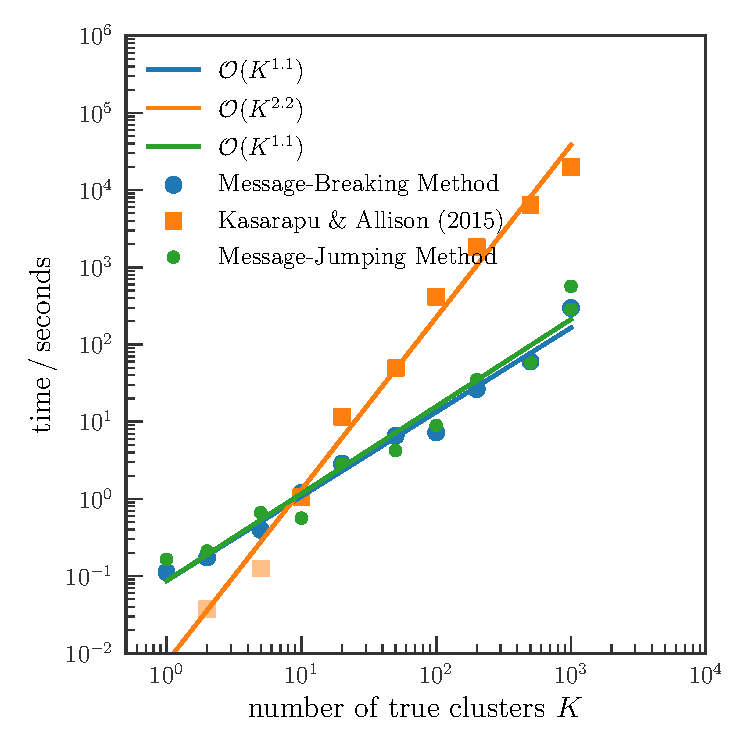
\includegraphics[width=1.0\textwidth]{cost.pdf}
    \caption{Elapsed wall clock time for trialled search strategies to converge 
             on generated datasets as a function of the true number of clusters
             in the data. The approximate cost functions are shown.}
    \label{fig:cost}
\end{figure}






\todo{Figure: corner plot showing chemical abundance data}

\todo{Figure: corner plot showing chemical abundance data, coloured by their responsibility}

\todo{Figures showing the concentration of chemically-identified data}



\todo{What do we find for the chemical abundance data}

\todo{Recovering known star clusters that are still gravitationally bound?}

\todo{Scientific insight from identifying groups in these data?}

\todo{Estimate of the number of star-forming sites in the galaxy?}



\section{References}
\bibliographystyle{elsarticle-num}
\bibliography{mmlbibliography}

\section{Appendices}
\subsection{The MML objective function}
\label{app:mml_derivation}
In the following subsections we provide expressions for the message length to
encode a gaussian mixture model, and our prior beliefs on the parameters of that model, before describing our
full objective function.

\subsubsection{The number of mixture components (or groups) $K$}

We assume a prior on the number of components $K$ of $\prior{K} \propto 2^{-K}$
\cite[][p279, sec. 6.8.2]{Wallace:2005} such that the length of the 
optimal lossless message to encode $K$ is 
\begin{equation}
    I(K) = -\log{\prior{K}} = K\log{2} + \textrm{constant} \quad .
\end{equation}
This  expresses our prior belief that there ought to be fewer components.



\subsubsection{The relative weight $w_k$ of each component}

We assume a uniform prior on the individual weights $\weight_{k}$. The weights
$\weights$ are drawn from a multinomial distribution, such that only $K - 1$
weights need to be encoded because $\sum_{k=1}^{K}\weight_k = 1$. Following
from Equation \ref{eq:taylor}, here we describe how our estimate of the message 
length of the multinomial parameter $\vec{\weight}$ quantifies the trade-off 
between stating the parameters $\vec{\weights}$ imprecisely, so as to keep the 
first part of the message short and place higher prior probability in the 
relevant uncertainty region, and the goodness-of-fit to the data, which is 
typically better if we state the estimates of the parameters more precisely. 
By balancing this trade-off, the length of this component is equal (within a 
small constant) to the negative log of the product of the prior probabilities 
of each group ($\prior{\vec{\weight}}$) divided by the square root of the 
expected Fisher information ($\sqrt{\fisher{\vec{\weight_k}}}$), where the 
Fisher information matrix contains the \emph{expected} second-order partial 
derivatives of the log-likelihood function. This describes how sharply the 
likelihood function peaks, and as a result it quantifies how precisely the 
parameters should be stated. In the case of uniform prior probabilities,
\begin{equation}
    \prior{\vec{\weight}} = (K - 1)! \quad ,
\end{equation}
\noindent{}the Fisher information is
\begin{equation}
\fisher{\vec{w}} = \frac{N^{K - 1}}{\prod_{k=1}^{K} w_k} \quad ,
\end{equation}
\noindent{}which gives the message length of this part to be
\begin{eqnarray}
I(\vec{w}) &=& -\log\left(\frac{\prior{\vec{w}}}{\sqrt{{\kappa_K}^K \fisher{\vec{w}}}}\right)  \nonumber \\
I(\vec{w}) &=& -\log{(K - 1)!} + \frac{K}{2}\log{\kappa_K} + \frac{K-1}{2}\log{N} - \frac{1}{2}\sum_{k=1}^{K}\log{\weight_k} \nonumber \\
I(\vec{w}) &=& -\log{\Gamma(K)} + \frac{K}{2}\log{\kappa_K} + \frac{K-1}{2}\log{N} - \frac{1}{2}\sum_{k=1}^{K}\log{\weight_k}
\end{eqnarray}
\noindent{}where $\kappa_K$ is a lattice constant that varies between $1/12$
and $1/(2\pi e)$ \cite{Boulton|Wallace:1969}.



\subsubsection{The mean $\vecmean_k$ and covariance matrix $\veccov_k$ for all
               $K$ Gaussian components}

In order to properly encode the means $\vecmean$ and covariance matrices
$\veccov$ for all $K$ mixtures, we must encode both our prior belief on 
those parameters and the determinant of the expected Fisher information 
matrix. For the $k$-th mixture the joint message length is
\begin{eqnarray}
  I(\vecmean_k,\veccov_k) &=& -\log{\left(\frac{\prior{{\vecmean_k,\veccov_k}}}{\sqrt{\detfisher{{\vecmean_k,\veccov_k}}}}\right)} \nonumber \\ 
  I(\vecmean_k,\veccov_k) &=& -\log{\prior{{\vecmean_k,\veccov_k}}} + \frac{1}{2}\log{\detfisher{{\vecmean_k,\veccov_k}}}
\end{eqnarray}

\noindent{}and for all mixtures:
\begin{equation}
  I(\vecmean,\veccov) = -\sum_{k=1}^{K}\log{\prior{{\vecmean_k,\veccov_k}}} + \frac{1}{2}\sum_{k=1}^{K}\log{\detfisher{{\vecmean_k,\veccov_k}}} \quad .
  \label{eq:I_component_params}
\end{equation}

We use an improper uniform prior on the mean $\vecmean$ for all mixtures such
that 
    $\mathcal{U}(\vecmean) = (-\infty, +\infty)$.
However,  the MML principle requires proper priors. In practice we make 
this prior proper by assuming the bounds on $\prior{\vecmean}$ are very large, but 
we do so without actually specifying the value of the bounds because they add 
only a constant value to the total message length.
We adopt a conjugate inverted Wishart prior for the covariance matrix of an
individual mixture \cite[Section 5.2.3 of][]{Knorr-Held:2000}:

\begin{equation}
  \prior{{\vecmean_k, \veccov_k}} \propto |\veccov_k|^{\frac{D+1}{2}} \quad .
  \label{eq:covariance-prior}
\end{equation}


% Casey: Reword following paragraph because it is clumsy.
Following Eq. \ref{eq:I_component_params}, we require the logarithm of the
determinant of the expected Fisher information matrix for $\vecmean_k$ and
$\veccov_k$ in order to encode the full message. In practice the determinant
of the Fisher information is non-trivial to evaluate, and as such we
approximate the determinant of the Fisher information
 $\detfisher{{\vecmean_k, \veccov_k}}$ 
as the product of $\detfisher{\vecmean_k}$ and $\detfisher{\veccov_k}$ 
\cite{oliver1996unsupervised,roberts1998bayesian}. In order to derive $\detfisher{\vecmean_k}$
we take the second derivative of the log-likelihood function 
$\likelihood(\data|\vectheta)$, which yields:
\begin{equation}
  \detfisher{\vecmean_k} = (N\weight_k)^{D}|\veccov_k|^{-1} \quad .
\end{equation}
We make use of an analytical expression for $\detfisher{\veccov_k}$
\cite{Dwyer:1967,Magnus|Neudecker:1988}:
\begin{equation}
  \detfisher{\veccov_k} = (N\weight_k)^\frac{D(D+1)}{2}2^{-D}|\veccov_k|^{-(D+1)} \quad .
\end{equation}
Combining these expressions gives our approximation for the determinant of
the expected Fisher information $\detfisher{{\vecmean_k,\veccov_k}}$:
\begin{eqnarray}
  \detfisher{{\vecmean_k,\veccov_k}} & \approx & \detfisher{\vecmean_k} \cdot \detfisher{\veccov_k} \nonumber \\
  \detfisher{{\vecmean_k,\veccov_k}} & \approx & (N\weight_k)^{D}|\veccov_k|^{-1}(N\weight_k)^\frac{D(D+1)}{2}2^{-D}|\veccov_k|^{-(D+1)} \nonumber \\
  \detfisher{{\vecmean_k,\veccov_k}} & \approx & (N\weight_k)^\frac{D(D+3)}{2}2^{-D}|\veccov_k|^{-(D+2)} \quad .
  \label{eq:mixture-component-det-fisher}
\end{eqnarray}


Substituting Eqs. \ref{eq:covariance-prior} and \ref{eq:mixture-component-det-fisher} 
into Eq. \ref{eq:I_component_params} gives the message length to encode the component
parameters $\vecmean$ and $\veccov$ for all $K$ mixtures:

\begin{eqnarray}
  I(\vecmean,\veccov) &=& -\sum_{k=1}^{K}\log{\prior{{\vecmean_k,\veccov_k}}} + \frac{1}{2}\sum_{k=1}^{K}\log{\detfisher{{\vecmean_k,\veccov_k}}} \nonumber \\
  I(\vecmean,\veccov) &=& -\sum_{k=1}^{K}\log{|\veccov_k|^{\frac{D + 1}{2}}}
    + \frac{1}{2}\sum_{k=1}^{K}\log{\left[(N\weight_k)^\frac{D(D+3)}{2}2^{-D}|\veccov_k|^{-(D+2)}\right]} \nonumber \\
%  I(\vecmean,\veccov) &=& \frac{D(D+3)}{4}\sum_{k=1}^{K}\log{N\weight_k} -\frac{(D + 1)}{2}\sum_{k=1}^{K}\log{|\veccov_k|}
    %-\frac{KD}{2}\log{2} \nonumber \\
%  && -\frac{D+2}{2}\sum_{k=1}^{K}\log{|\veccov_k|} \nonumber \\
  I(\vecmean,\veccov) &=& \frac{D(D+3)}{4}\sum_{k=1}^{K}\log{N\weight_k} -\frac{2D+3}{2}\sum_{k=1}^{K}\log{|\veccov_k|} - \frac{KD}{2}\log{2} 
\end{eqnarray}


\subsubsection{The data given the model}
If we assume that the data have homoskedastic noise properties, then the 
precision of each measurement $\mathcal{E}$ relates the probability of a
datum $p(\datum_n)$ can be related to the probability density of
the datum, given the model 
$p(\datum_n) = \mathcal{E}^{D}p(y_i|\mathcal{M})$.
In this work we adopt $\mathcal{E} = 0.01$, but we note that the value of
$\mathcal{E}$ has no effect on our inferences.  The message length of encoding
a datum given the model is,
\begin{equation}
  I(\data_n) = -\log{p(\data_n)} = -D\log\mathcal{E} - \log\sum_{k=1}^{K}\weight_{k}f_{k}(\data_n|\vecmean_k,\veccov_k)
\end{equation}

\noindent{}and for the entire data:
\begin{eqnarray}
  I(\data|\vectheta) &=& -ND\log\mathcal{E} - \sum_{n=1}^{N}\log\sum_{k=1}^{K}w_{k}f_k(\data_n|\vecmean_k,\veccov_k) \quad .
\end{eqnarray}

The final part of the message is to encode the lattice quantisation constant,
which arises from the approximation to the (so-called) strict MML, where
parameters are quantised into intervals in high dimensional space in order to
be losslessly encoded.  We use an approximation of the lattice constant
\citep[see Sections 5.1.12 and 3.3.4 of ]
%[]
{Wallace:2005} such that,
\begin{equation}
  \log\kappa(Q) = \frac{\log{Q\pi}}{Q} - \log{2\pi} - 1 \quad ,
\end{equation}

\noindent{}where $Q$ is the total number of free parameters in the model. Each
Gaussian component in the mixture requires $D$ parameters to specify $\vecmean$,
and a covariance matrix with off-diagonal terms requires $\frac{1}{2}D(D+1)$ 
parameters. Because only $K - 1$ weights need to be encoded, the total number of free
parameters is
\begin{equation}
    Q = K\left[\frac{D(D+3)}{2} + 1\right] - 1 \quad .
    \label{eq:number-of-parameters}
\end{equation}


\subsection{Objective function}

Combining the expressions for the message length (or information content) of
each component, we arrive at our objective function $I$ to minimise across 
all model parameters (including the number of mixtures, $K$):
\begin{eqnarray}
	I(\vec{\data}|\vec{\psi}, N, D) &=& -\log\mathcal{L}\left(\vec{\data}|\vectheta\right) - \frac{(D + 2)}{2}\sum_{k=1}^{K}\log{|{\cov}_k|} \nonumber \\
	&& \cdots\ + \left(\frac{D(D+3)}{4} - \frac{1}{2}\right)\sum_{k=1}^{K}\log{\weight_k} + K\left(1-\frac{D}{2}\right)\log{2} \nonumber \\ && \cdots\ + \log\Gamma{(K)} + \frac{1}{2}\left(\log{Q\pi} - Q\log{2\pi}\right) + \frac{Q}{2}\log{N} \,\,\,\, . 
	\label{eq:objective_function}
\end{eqnarray}



\section{Bounds on components of the message length}

Developing similar theoretical bounds for $I_2$ is not straightforward, because
the determinants of the covariance matrices of Gaussian components will not
-- to our knowledge -- strictly follow some expected distribution, in the way 
that the weights $\weights$ follow a multinomial distribution. Similarly, the
\emph{scale} of $|\veccov_k|$ will depend entirely on the distribution of the
data. In that sense, we cannot a priori state with any certainty about what 
values $|\veccov_k|$ might take (or $\log{|\veccov_k|}$) without knowing
something about the data first. Even demanding that the covariance matrices
$\veccov_k$ are positive semi-definite only informs us that $\log{|\veccov_k|}$
is finite. However, there are quantitative predictions we can make on the 
bounds of $\sum_{k=1}^{K}\log{|\veccov_k|}$ if something is known about the
data. Specifically if we consider the determinant of the sample covariance 
matrix, which we denote $|\cov_{u}|$ (where the $u$ subscript denotes `upper',
for the upper limit on the covariance matrix), then we can state with confidence that
the sample covariance matrix describes the maximum amount of variance that 
could be captured by the components in the mixture. For example, a limiting
case of $\sum_{k=1}^{K}\log{|\veccov_k|}$ can be described when the determinant
of the sample covariance matrix must be equally (uniformly) captured by $K$ 
components in a mixture. In other words, the maximum variance in the data 
must be equally spread between the components in the mixture. Uniformly 
describing the variance in the data is the limiting case because any 
non-uniformity would lead to smaller $|\veccov|$ for one mixture (and larger 
for another), and that asymmetry would lead to a higher $I_2$ because 
$\log(x - \epsilon) + \log(x + \epsilon) < 2\log{x}$, and because of the 
$-(1 + \frac{D}{2})$ term that enters multiplicatively in the calculation of 
$I_2$. Thus, we can specify a lower bound on $I_2$ based on the determinant of
the sample covariance matrix $|\cov_{u}|$:

\begin{eqnarray}
    I_{2} & \geq & -\left(1 + \frac{D}{2}\right)\sum_{k=1}^{K}\log{\frac{|\cov_u|}{K}} \nonumber \\
    I_{2} & \geq & -\left(1 + \frac{D}{2}\right)\left(K\log{|\cov_u|} - K\log{K}\right) 
\end{eqnarray}


The other extreme on $I_2$ can be approximated by estimating the \emph{minimum}
possible variance that could be captured by any single component. In theory
this approaches zero, but in practice it will be set by the minimum pairwise
distance in $D$ dimensions. Specifically, if we consider two data points to be
captured by a component in the mixture, an those two data points are the
closest two data points (in high dimensional space) of any data points, then
the variance captured by that Gaussian component will represent the \emph{minimum}
possible variance that can be captured by any single component.  
In practice we calculate the minimum total pair-wise euclidean distance $d_{min}$
in $D$ dimensions, average it over the dimensions, and approximate the minimum
determinant of the covariance matrix $|\cov_l|$ as
\begin{equation}
    |\cov_{l}| \approx \prod_{d=1}^{D}\left(\frac{d_{min}}{2}\right)^2 \quad ,
\end{equation}
\noindent{}which approximately represents the variance between two data points,
but ignores correlations and assumes only a mean distance in $D$ dimensions
(for comuptational cost). With these approximations,
\begin{eqnarray}
    \log{|\cov_{l}|} & \approx & \sum_{d=1}^{D}\log{\left(\frac{d_{min}}{2}\right)^2}  \nonumber \\
    \log{|\cov_{l}|} & \approx & 2D\log{\left(\frac{d_{min}}{2}\right)} \quad ,
\end{eqnarray}
\noindent{}and the upper limit on $I_2$ is:
\begin{eqnarray}
    I_{2} & \leq & -\left(1 + \frac{D}{2}\right)\sum_{k=1}^{K}\log{|\cov_l|} \nonumber \\
    I_{2} & \leq & -DK\left(D+2\right)\log{\left(\frac{d_{min}}{2}\right)} \quad .
\end{eqnarray}

Here our bounds on $I_2$ are only dependent on $K$, $D$, the minimum euclidean
pair-wise distance $d_{min}$, and the determinant of the sample covariance
matrix $|\cov_u|$. In practice it is the lower bound on $I_{2}$ that is 
arguably more useful for search and optimisation, but one could conceive
situations where there is great utility in also having upper bounds on $I_1$
and $I_2$.

There is no finite upper bound on $I_{3}$ because the negative log-likelihood
$-\log\likelihood$ will approach infinity for an increasingly poor fit to the
data. A useful lower limit, however, does exist. The negative log-likelihood
in Eq. \ref{eq:log-likelihood} can be expanded as,
\begin{equation}
    -\log\mathcal{L}\left(\vec{\data}|\vec{\theta}\right) = \sum_{n=1}^{N}\log\sum_{k=1}^{K}\frac{\weight_k}{\sqrt{(2\pi)^{D}|\vec{\cov}_k|}}\exp\left[-\frac{1}{2}\left(\vec{\data}_n - \vecmean_k\right)^\intercal{}\vec{\cov}_{k}^{-1}\left(\vec{\data}_n - \vecmean_k\right)\right]
\end{equation}
\noindent{}and we can define
\begin{equation}
\chi^{2}_{nk} = \left(\vec{\data}_{n} - \vecmean_{k}\right)^\intercal{}\vec{\cov}_{k}^{-1}\left(\vec{\data}_{n} - \vecmean_{k}\right) \quad .
\end{equation}
For the sake of placing a lower bound on $I_{3}$, let us assume that each data
point will be `mostly' explained by one of the components in the 
mixture\footnote{We model the data with partial assignment, but here we merely 
seek to place a lower bound on the negative log-likelihood.}, but we do not 
necessarily know which component, or what the parameters of that component are. 
In that situation, we can state that the component that \emph{does} explain
the data will have $\chi_{nk}^2 \sim \textrm{O}\left(D\right)$ and $\exp(-\frac{1}{2}\chi^2) \rightarrow 1$
whereas the other components that do not explain the data will have 
$\chi_{nk}^2 >> D$ such that $\exp(-\frac{1}{2}\chi^2) \rightarrow 0$. With
this simplification we can write an approximation for the negative log-likelihood
that does not require knowledge about which data points are associated to what
component, because the number of times that the expression $\exp(-\frac{1}{2}\chi^2)$
will be non-zero is for the $k$th mixture component will be $N\weight_k$. The
approximate lower bound is:
\begin{eqnarray}
    -\log\likelihood\left(\vec{\data}|\vec{\theta}\right) & \gtrsim & -\sum_{k=1}^{K}N\weight_{k}\log\left[\frac{\weight_k}{\sqrt{(2\pi)^{D}|\vec{\cov}_k|}}\exp\left(-\frac{1}{2}{D}\right)\right] \\
    -\log\likelihood\left(\vec{\data}|\vec{\theta}\right) & \gtrsim & -N\sum_{k=1}^{K}\weight_{k}\log{\weight_k} + \frac{1}{2}N\sum_{k=1}^{K}\weight_{k}\log{|\vec{\cov}_k|} + \frac{1}{2}ND\left(1 + \log{2\pi}\right) \quad . \nonumber
    \label{eq:logl-lower-bound}
\end{eqnarray}
\noindent{}Like before, we can consider the lower bound on $-N\sum_{k=1}^{K}\weight_{k}\log\weight_k$
for any mixture of $K$ components by setting the weight of $K - 1$ mixtures
to the smallest realistic values, where those mixtures encapsulate only two
data points and $w_{1} = w_2 = w_{\cdots} = w_{K-1} = 2/N$ such that
%\begin{eqnarray}
%	\sum_{k=1}^{K}\weight_{k}\log\weight_k = \left[(K-1)\left(\frac{2}{N}\log{\frac{2}{N}}\right) + \left(1-\frac{2(K-1)}{N}\right)\log{\left(1-\frac{2(K-1)}{N}\right)}\right] \nonumber
%\end{eqnarray}`
%\noindent{}and
\begin{eqnarray}
	-N\sum_{k=1}^{K}\weight_{k}\log\weight_k \geq 2(1-K)\log{2} + N\log{N} - (N-2K+2)\log{\left(N - 2K + 2\right)}
\end{eqnarray}
%  log(a-b) = log(a) + log(1 - b/a)
% log(1 - b/a) = log(a-b) - log(a)
% log(1 - b/a) = log(N - 2K + 2) - log(N)

% 2(1-K)log(2) - 2(1-K)log(N) + (2K - N - 2)log(N - 2K + 2) - (2K - N - 2)log(N)
% 2(1-K)log(2) - 2log(N) + 2Klog(N) + (2K - N - 2)log(N - 2K + 2) - (2K - N - 2)log(N)
% 2(1-K)log(2) + (2K - 2)log(N) + (2K - N - 2)log(N - 2K + 2) - (2K - 2 - N)log(N)
% 2(1-K)log(2) + Nlog(N) + (2K - N - 2)log(N - 2K + 2)



The remaining term in Eq. \ref{eq:logl-lower-bound}, $\frac{1}{2}N\sum_{k=1}^{K}\weight_{k}\log|\vec{\cov}_k|$, requires some  consideration.

\andy{here}


\subsection{Reproducibility} \label{sec:reproducibility}

\noindent{}This project was developed in a public \texttt{git} repository that is 
accessible at:
\begin{center}
\giturl
\end{center}
\noindent{}This repository includes a well-tested \texttt{Python 3.6} implementation
of the algorithms described here, scripts to reproduce our results, and \LaTeX\ to compile this manuscript. This research can be reproduced in full using
the following commands in a modern terminal:\\\\
\bashcommand{git clone https://github.com/andycasey/gmmmml.git gmmmml}
\bashcommand{cd gmmmml/}
\bashcommand{git checkout \githash}
\bashcommand{./reproduce}

Reproducing these results will require at least \todo{X}\,Gb of free disk space
and \todo{Y}\,hours of compute time, mostly because of the extensive algorithm 
comparisons performed.

\subsubsection{Search Strategy Implementation}

The astute reader will recognise that each search `strategy' we have described
is implemented in the \texttt{gmmmml} codebase as a set of `policies' that govern
different behaviour of the search:
\begin{itemize}
\item \emph{Initialisation}: how many mixtures should be initialised, and how?
\item \emph{Prediction}: when should we make predictions about the message length of future mixtures, and how far ahead should we make predictions?
\item \emph{Movement}: \emph{what} should the next $K$ be?
\item \emph{Repartition}: \emph{how} should we move to the next $K$? Should we repartition an existing mixture, initialise a new mixture, or should we make a probabilistic decision?
\item \emph{Convergence}: when should we stop searching?
\end{itemize}

As an example, the \emph{Message-Breaking Method} can equivalently be described
by a set of policies that: 
	\emph{initialise} a single mixture $K = 1$; 
	makes no \emph{predictions};
	\emph{moves} a single step towards the minimum message length;
	\emph{repartitions} the closest existing mixture by splitting the component with the maximum message length; and 
	describes \emph{convergence} at the point when the message length of the current mixture is worse than the previous mixture. 
This policy-strategy factorisation allows for the trivial implementation of flexible search strategies with complex behaviour. We encourage the development of new search strategies.



%---------
% COMMENTS
%---------


\begin{comment}
We employ two criteria for comparing the proposed search methods to the benchmark: the message length and the Kullback Leibler divergence~\cite{kullback1951information}.

\paragraph{Message Length}

\paragraph{Kullback Leibler divergence}
\end{comment}


\begin{comment}

\subsection{The MML$_{K+D}$ Method}
Say we wanted to calculate whether another mixture was warranted. If another
mixture were preferred then we would want:

\begin{eqnarray}
  \Delta{}I_{K+1} - I_{K} < 0
\end{eqnarray}

The expression is given as:
\begin{eqnarray*}
\Delta{I_{K+1} - I_K} & = & (K + 1)\log{2} - K\log{2} \\ % I_k^(new) - %I_k^(old)
  &&+ \frac{(K)}{2}\log{N} - \frac{1}{2}\sum_{k=1}^{K+1}\log{w_k}^{(new)} - \log{|\Gamma(K+1)|} \\ % I_w^(new)
  &&- \frac{(K - 1)}{2}\log{N} + \frac{1}{2}\sum_{k=1}^{K}\log{w_k} + \log{|\Gamma(K)|}\\ % I_w^(old)
  &&+ \mathcal{L}^{(new)} - DN\log{y_{err}} \\ % Likelihood (new)\\
  &&- \mathcal{L}^{(old)} + DN\log{y_{err}} \\ % Likelihood (old) \\
  &&+ \frac{1}{2}\sum_{k=1}^{K+1(new)}\left[\frac{D(D+3)}{2}\log{{Nw_k}} - (D + 2)\log{|\veccov_k|} - D\log{2}\right] \\ % I_t^(new)
  &&- \frac{1}{2}\sum_{k=1}^{K(old)}\left[\frac{D(D+3)}{2}\log{{Nw_k}} - (D + 2)\log{|\veccov_k|} - D\log{2}\right] \\ % I_t^(old)
  &&- \frac{Q^{(new)}}{2}\log(2\pi) + \frac{\log{Q^{(new)}\pi}}{2} \\ % lattice, minus the lattice of part 2
  &&+ \frac{Q^{(old)}}{2}\log(2\pi) - \frac{\log{Q^{(old)}\pi}}{2} % lattice, minus the lattice of part 2
\end{eqnarray*}

\noindent{}By making use of $\log{\Gamma(K)} - \log{\Gamma(K + 1)} = -\log{K}$ and re-arranging the expression:

\begin{eqnarray}
\Delta{}I_{K+1} - I_K &=& \log{2} % \Delta{}I_k
    + \frac{1}{2}\log{N} - \log{K} - \frac{1}{2}\left(\sum_{k=1}^{K+1}\log{w_k^{(new)}} - \sum_{k=1}^{K}\log{w_k^{(old)}}\right) \nonumber \\ % \Delta{}I_w
& +& \mathcal{L}^{(new)} - \mathcal{L}^{(old)} \nonumber \\ % likelihood
& +& \frac{1}{2}\left[\frac{D(D+3)}{2}\left(\sum_{k=1}^{K+1}\log{Nw_k^{(new)} - \sum_{k=1}^{K+1}\log{Nw_k^{(old)}}} \right) \right.\nonumber\\
&-& \left.\left(D+2\right)\left(\sum_{k=1}^{K+1}\log{|\veccov_k|^{(new)}} - \sum_{k=1}^{K+1}\log{|\veccov_k|^{(old)}}\right)\right] \nonumber \\
& +& \frac{\log(2\pi)}{2}(Q^{(old)} - Q^{(new)}) + \frac{\pi}{2}\left(\log{Q^{(new)}} - \log{Q^{(old)}}\right)
\label{eq:13}
\end{eqnarray}

Expanding the $Q$ terms:

\begin{eqnarray}
Q^{(old)} - Q^{(new)} &=& \frac{1}{2}DK(D + 3) + K - 1 - \frac{1}{2}D(K + 1)(D + 3) + (K + 1) - 1 \nonumber \\
Q^{(old)} - Q^{(new)} &=& -\frac{1}{2}D(D+3) + 2K  - 1
\label{eq:14}
\end{eqnarray}

\noindent{}And making use of the following logarithmic identities,
\begin{eqnarray}
  \log{Q^{(new)}} &=& \log{\left(\frac{1}{2}D(K+1)(D + 3) + K\right)} \nonumber \\
                  &=& \log{\left(\frac{1}{2}D(K+1)(D + 3)\right)} + \log{\left(1 + \frac{K}{\frac{1}{2}D(K+1)(D + 3)}\right)} \\
  \log{Q^{(old)}} &=& \log{\left(\frac{1}{2}DK(D + 3) + K - 1\right)} \nonumber \\
                  &=& \log{\left(\frac{1}{2}DK(D + 3)\right)} + \log{\left(1 + \frac{K - 1}{\frac{1}{2}DK(D + 3)}\right)}
\end{eqnarray}


\noindent{}gives us,

\begin{eqnarray}
  \log{Q^{(new)}} &- \log{Q^{(old)}} = \log{\left(\frac{1}{2}D(K+1)(D + 3)\right)} - \log{\left(\frac{1}{2}DK(D + 3)\right)} \nonumber \\
                                    &+ \log{\left(1 + \frac{K}{\frac{1}{2}D(K+1)(D + 3)}\right)} - \log{\left(1 + \frac{K - 1}{\frac{1}{2}DK(D + 3)}\right)}.
\end{eqnarray}
The second row of terms can be ignored because they are very small (typically less than 1 bit). This is because as $K \rightarrow \infinity$, $2K/D(K+1)(D+3) \rightarrow 1$, thus $\log{\left(1 + \frac{K}{\frac{1}{2}D(K+1)(D + 3)}\right)} \rightarrow \log{2}$. Similarly as $D \rightarrow \infinity$, $2K/D(K+1)(D+3) \rightarrow 0$.

As $K \rightarrow \infinity$ then $2(K-1)/DK(D+3) \rightarrow 1$ and as $D \rightarrow \infinity$ then $2(K-1)/DK(D+3) \rightarrow 0$ and thus $\log{\left(1 + \frac{K - 1}{\frac{1}{2}DK(D + 3)}\right)} \approx 0$.

\noindent{}Ignoring these minor terms:

\begin{eqnarray}
  \log{Q^{(new)}} - \log{Q^{(old)}} &\approx& \log{\left(\frac{1}{2}D(K+1)(D + 3)\right)} - \log{\left(\frac{1}{2}DK(D + 3)\right)} \nonumber \\
  \log{Q^{(new)}} - \log{Q^{(old)}} &\approx& \log{(K + 1)} - \log{K}
  \label{eq:19}
\end{eqnarray}

\noindent{}Substituting Eqs. \ref{eq:19} and \ref{eq:14} into \ref{eq:13} yields:

\begin{eqnarray}
\Delta{}I_{K+1} &-& I_K \approx \log{2} % \Delta{}I_k
    + \frac{1}{2}\log{N} - \log{K} - \frac{1}{2}\left(\sum_{k=1}^{K+1}\log{w_k^{(new)}} - \sum_{k=1}^{K}\log{w_k^{(old)}}\right) \nonumber \\ % \Delta{}I_w
& +& \mathcal{L}^{(new)} - \mathcal{L}^{(old)} \nonumber \\ % likelihood
& +& \frac{1}{2}\left[\frac{D(D+3)}{2}\left(\sum_{k=1}^{K+1}\log{Nw_k^{(new)} - \sum_{k=1}^{K+1}\log{Nw_k^{(old)}}} \right) \right.\nonumber \\
&-& \left.\left(D+2\right)\left(\sum_{k=1}^{K+1}\log{|\veccov_k|^{(new)}} - \sum_{k=1}^{K+1}\log{|\veccov_k|^{(old)}}\right)\right] \nonumber \\
& +& \frac{\log(2\pi)}{2}(-\frac{1}{2}D(D+3) + 2K  - 1) + \frac{\pi}{2}\left(\log{(K + 1)} - \log{K}\right)
\end{eqnarray}
\end{comment}


\begin{comment}
\subsection{Method of Moments}
% \alda{This is a copy paste from David's email with minor changes}
%
% Re the case of two (or more) classes with the same mean:
% In 2D, a simple case in point is two classes with the same mean
% such that $\sigma_{1, x} = \sigma_{2, y} >> \sigma_{2, x} = \sigma_{1, y}$.
% Andy said that this and higher dimensional stuff can be picked up
% by dropping to 1 dimension along the eigenvector of largest eigenvalue.
%
%
% I wonder also about the merits of dropping to 2 dimensions (if we have at least 2 attributes), being the eigenvectors of the two largest eigenvalues. 
%
% One could possibly check whether uniform radially directly from the original 2D projection without having to project it to a circle (i.e., it might be pretty easy to work out what the angle of each point would be post-transformation without having to do the transformation).  The 2D projection is 1D in the sense that we only care about the angle around the circle.  And then some test (e.g., Kolmogorov-Smirnov test) for whether data is uniform in radial distribution.  If not uniform, then perhaps grounds for splitting.
%
% Re looking at things in 1 dimension (not 2D followed by 1D [0, 2 pi) angle
% as above but rather projecting on eigenvector of largest eigenvalue), we
% discussed moments - e.g., \url{https://en.wikipedia.org/wiki/Normal_distribution}.
% So, 2nd, 4th, 6th and 8th moments of a true Gaussian are 1, 3, 15, 105.
%

We informally outline here the method of moments form of search heuristic and then look at how it might be applied.

Let's suppose we have a 1D component.  We'll shift it (without loss of generality, w.l.o.g.) so that its mean is 0 and we'll shrink or expand it (again, w.l.o.g.) so that its s.d. ($\sigma$) is 1 (and variance v is 1).
We consider now splitting it into K components with mean 0,
mixing weights (or proportions) $w_1, ..., w_i, ..., w_K$ and s.d.s $\sigma_i$ (and variances $v_i = (\sigma_i)^2$).
Let's set $K = 2$, so $w_2 = 1 - w_1$.

Noting that the 2nd, 4th, 6th and 8th moments of a true Gaussian distribution are 1, 3, 15, 105,
suppose the moments of our current component are 1, $3 \alpha_4, 15 \alpha_6$ and $105 \alpha_8, ... $.
We get some equations - if we have the correct number of equations,
they're simultaneous equations.

If we get too many equations (by using too many moments), then it
becomes something of a fitting or regression problem to choose
$w_1, ..., w_i, ..., w_K$ and s.d.s $\sigma_i$, variances $v_i = (\sigma_i)^2$.

Our simultaneous equations are:

\begin{align*}
w_1 v_1       + (1 - w_1) v_2       &=    1\\
w_1 (v_1)^2  + (1 - w_1) (v_2)^2  &=    3 \alpha_4\\
w_1 (v_1)^3  + (1 - w_1) (v_2)^3  &=   15 \alpha_6\\
w_1 (v_1)^4  + (1 - w_1) (v_2)^4  &=  105 \alpha_8
\end{align*}

% These might be messy to solve on the fly  but one could pre-process by solving many of these beforehand (actually, approximately solving these beforehand, as it's only
% a heuristic, anyway) at the very start of the program while loading in the data.

So, for $1000 \times 1000 = 10^6$ different values of $\alpha_4$ and $\alpha_6$
or for $100 \times 100 \times 100 = 10^6$ different values of $\alpha_4, \alpha_6$ and $\alpha_8$
one could pre-compute {\em approximate} 1,000,000ish `solutions' to the above simultaneous equations.

Then, when running the program with real actual values of $\alpha_4$ and $\alpha_6$ (and $\alpha_8$),
one could just grab something from nearby in this pre-computed look-up table
as putative values for $w_1, v_1, v_2$ (and etc., if need be).

% As an example of this algorithm, consider the mixture $0.6 N(-3, 2^2) + 0.4 N(7, 3^2)$.
% The best fitting single Normal distribution to this would be $N(1, \sqrt{30}^2)$.
%
As an
% another
example of this algorithm, consider a first moment of $0$, a $2^{\rm nd}$ moment of $6$ and a $4^{\rm th}$ moment of $3 \times 37.2 = 111.6$.
Solving the simultaneous equations gives us $0.6 N(0, 2^2) +  0.4 N(0, 3^2)$.
\end{comment}

\begin{comment}
\subsection{The k-means++ algorithm}

The k-means++ algorithm extends the k-means method with an efficient way of choosing centres. Let $D(x)$ denote the shortest distance from a data point $x$ to the closest centre that has already been selected. The k-means++ has the following steps:

\begin{enumerate}
    \item Selects a centre $c_1$ uniformly at random from the $N$ data points.
    \item Selects a new centre $c_i$ from the data points with probability $\frac{D(x)^2}{\sum_{x\in X}}D(x)^2$
    \item Repeat Step 2. until k centres have been selected.
    \item Proceed as with the standard k-means algorithm.
\end{enumerate}

k-means++ is $O(\log k)$-Competitive.
\end{comment}




\end{document}
